\documentclass[12pt]{article}
\usepackage[utf8]{inputenc}
\usepackage{amssymb}
\usepackage{graphicx}
\graphicspath{{images/}}

\title{AI1110 Assignment 1}
\author{Dasari Srinith (cs21btech11015)}
\date{29 March, 2022}

\setlength{\parindent}{0cm}
\usepackage{parskip}
\pagenumbering{gobble}
\begin{document}

\maketitle
\section*{Paper 2018}

\section*{Q4 (c)}

    Solve $x^2 + 7x = 7$ and give your answer correct to two decimals.
    
\section*{Solution}

    Given,\\
    To Find the roots of $x^2 +7x -7 = 0$.
    
    We know that for the quadratic equation of form $ax^2 + bx +c = 0$,\\
    the roots are
               $$\displaystyle\frac{-b+\sqrt{b^2 -4ac}}{2a}
                       ,\displaystyle\frac{-b-\sqrt{b^2 -4ac}}{2a}$$
                       
    $\Rightarrow$ The roots are $\displaystyle\frac{-7+\sqrt{49 -4(1)(-7)}}{2(1)}
                       ,\displaystyle\frac{-7-\sqrt{49 -4(1)(-7)}}{2(1)}$
                       
    $\Rightarrow$ The roots are $\displaystyle\frac{-7+\sqrt{77}}{2}
                       ,\displaystyle\frac{-7-\sqrt{77}}{2}$
                       
    $\Rightarrow$ The roots are $\displaystyle\frac{-7+8.7749}{2}
                       ,\displaystyle\frac{-7-8.7749}{2}$\\
    ($\sqrt{77}$ can be found by long division method up to four decimals)
                       
    $\Rightarrow$ The roots are -7.8874, 0.8874
    
    On rounding them off to 2 decimal places we get the roots as -7.89 and 0.89.
    
    \begin{figure}
        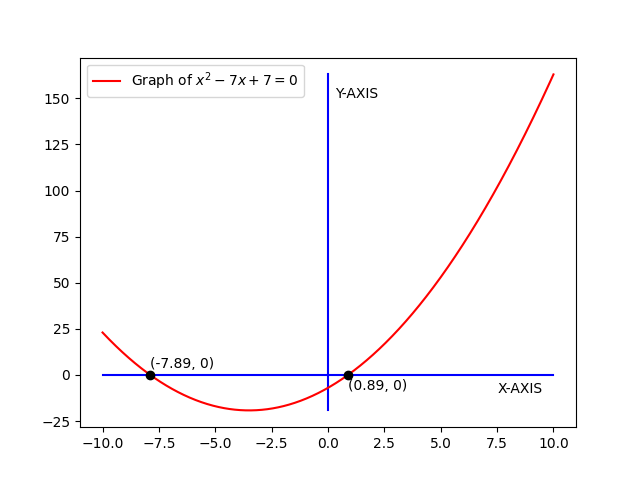
\includegraphics[width=\textwidth]{plot.png}
        \caption{Plot showing the polynomial in $x^2 +7x -7 = 0$}
    \end{figure}
    
    $\therefore$ The solutions of $x^2 + 7x = 7$ are  $x = -7.89$ and $x = 0.89$.
    
\end{document}
